\documentclass[aspectratio=169, 12pt, xcolor={dvipsnames,table}]{beamer}
\usetheme{metropolis}
\usepackage{amsmath, amssymb}
\usepackage{array, booktabs}
\usepackage{tikz}

% --- Color tags --------------------------------------------------------
\definecolor{wbox}{RGB}{240,240,240}
\definecolor{gbox}{RGB}{150,150,150}
\definecolor{bbox}{RGB}{40,40,40}
\definecolor{accent}{RGB}{200,50,50}
\definecolor{hint}{RGB}{120,120,120}

\newcommand{\ctag}[3]{%
  \tikz[baseline=-0.6ex]\node[rectangle,draw=black,fill=#1,
    minimum width=5mm,minimum height=5mm,inner sep=0pt,line width=0.3pt]
    {\scriptsize\color{#2}\textbf{#3}};}
\newcommand{\W}{\ctag{wbox}{black}{W}}
\newcommand{\Gr}{\ctag{gbox}{white}{G}}
\newcommand{\Bl}{\ctag{bbox}{white}{B}}

\newcommand{\ans}[1]{\textcolor{accent}{\textbf{#1}}}
\newcommand{\hintline}[1]{\vfill\begin{center}\small\textcolor{hint}{#1}\end{center}}

\title{The Colored Restaurant Row}
\subtitle{A game that motivates the Bellman equation}
\date{}

\begin{document}

\maketitle

% ======================================================================
\begin{frame}{The game}
\large
You are walking home past \textbf{8 restaurants}. At each one:
\begin{enumerate}
  \item You see the restaurant's \textbf{color tag}: \W\ \Gr\ or \Bl.
  \item You decide \textbf{EAT} or \textbf{SKIP}.
  \item The \textbf{rating} (1--10) is then revealed.
  \item If you ate, add the rating to your score.
\end{enumerate}
\vfill
\begin{center}
\large You have only \textbf{3 EAT slots} across the 8 restaurants.\\[0.3em]
Maximize your total rating.
\end{center}
\end{frame}

% ======================================================================
\begin{frame}{Rules --- one screen}
\large
\begin{itemize}
  \item 8 restaurants. Color announced \emph{first}, then you commit, then the rating is revealed.
  \item At most \textbf{3 EATs} total.
  \item Score = sum of ratings where you EAT.
  \item \textbf{25 seconds} per decision.
  \item You will play \textbf{twice} --- with fresh sequences drawn from the same hidden process.
\end{itemize}
\hintline{The color is a clue. What it means is up to you to figure out.}
\end{frame}

% ======================================================================
\begin{frame}{Your paper strip}
\centering
\small
\renewcommand{\arraystretch}{1.3}
\begin{tabular}{|c|c|c|c|c|c|}
\hline
\# & Color & Rating & EAT / SKIP & Slots left & Score \\
\hline
1 & & & & 3 & 0 \\ \hline
2 & & & & & \\ \hline
\multicolumn{6}{|c|}{$\cdots$} \\ \hline
8 & & & & & \\ \hline
\end{tabular}
\vspace{1em}

\textbf{Color tally panel} --- fill it as ratings are revealed:

\vspace{0.3em}
\begin{tabular}{|c|c|c|c|}
\hline
Color & Count & Sum of ratings & Mean \\ \hline
\W\ white & & & \\ \hline
\Gr\ gray  & & & \\ \hline
\Bl\ black & & & \\ \hline
\end{tabular}
\hintline{Every rating you see --- EAT or SKIP --- updates the tally. The tally is your memory.}
\end{frame}

% ======================================================================
\begin{frame}{\Large Play 1}
\vfill
\begin{center}
{\Huge Ready?}\\[1em]
\large Color $\to$ decide $\to$ rating. 3 slots, 8 restaurants.\\[0.3em]
\textcolor{hint}{Keep your tally panel up to date.}
\end{center}
\vfill
\end{frame}

% ======================================================================
\begin{frame}{After Play 1 --- pool the class}
\large
\begin{itemize}
  \item Put your final score on a sticky note $\to$ class histogram.
  \item Read out your running color means:
  \begin{center}
    \W\ mean, \ \Gr\ mean, \ \Bl\ mean.
  \end{center}
  \item Together we have $\sim\!25 \times 8 = 200$ observations. What's the pattern?
\end{itemize}
\hintline{Individually you saw 2--3 of each color. Together we have a much sharper picture.}
\end{frame}

% ======================================================================
\begin{frame}{Reveal --- the hidden regularity}
\large
The rating at each restaurant is drawn from a fixed distribution \emph{conditional on its color}:
\vfill
\begin{center}
\renewcommand{\arraystretch}{1.4}
\begin{tabular}{c l c c}
\toprule
Color & Distribution & $\mathbb{E}[r \mid \text{color}]$ & Informal \\
\midrule
\W\ white & Uniform on $\{1, 2, 3, 4\}$         & $2.5$ & cheap diner \\
\Gr\ gray  & Uniform on $\{3, 4, 5, 6, 7\}$     & $5.0$ & middling \\
\Bl\ black & Uniform on $\{6, 7, 8, 9, 10\}$    & $8.0$ & high-end \\
\bottomrule
\end{tabular}
\end{center}
\vfill
\hintline{Same distributions in Play 2. Your tally \emph{is} your estimate of the table above.}
\end{frame}

% ======================================================================
\begin{frame}{\Large Play 2 --- with what you now know}
\vfill
\begin{center}
{\Huge Round 2.}\\[1em]
\large Same rules, fresh sequence, same hidden distributions.\\[0.3em]
\textcolor{hint}{What's your policy now?}
\end{center}
\vfill
\end{frame}

% ======================================================================
\begin{frame}{After Play 2 --- compare histograms}
\begin{columns}[T]
\column{0.5\textwidth}
\centering
\textbf{Play 1}\\[0.5em]
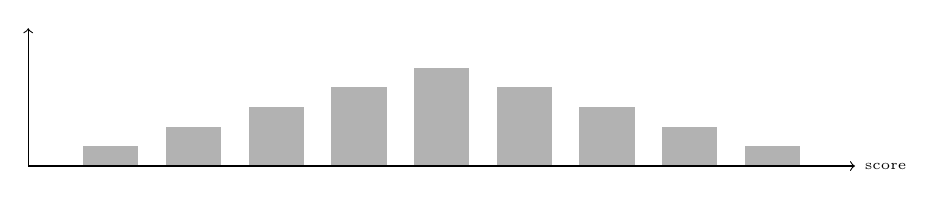
\begin{tikzpicture}[xscale=0.35, yscale=0.25]
  \foreach \x/\h in {5/1, 8/2, 11/3, 14/4, 17/5, 20/4, 23/3, 26/2, 29/1}
    \fill[gray!60] (\x,0) rectangle (\x+2,\h);
  \draw[->] (3,0) -- (33,0) node[right]{\tiny score};
  \draw[->] (3,0) -- (3,7);
\end{tikzpicture}\\
\small wide, greedy-dominated

\column{0.5\textwidth}
\centering
\textbf{Play 2}\\[0.5em]
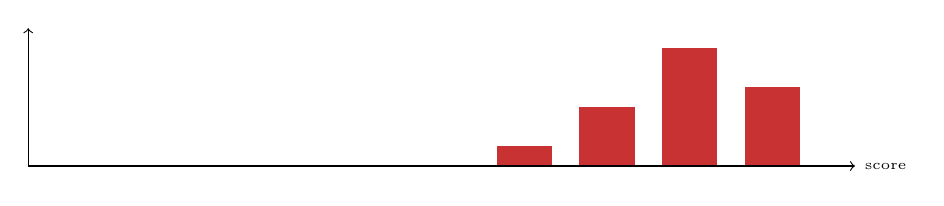
\begin{tikzpicture}[xscale=0.35, yscale=0.25]
  \foreach \x/\h in {20/1, 23/3, 26/6, 29/4}
    \fill[accent] (\x,0) rectangle (\x+2,\h);
  \draw[->] (3,0) -- (33,0) node[right]{\tiny score};
  \draw[->] (3,0) -- (3,7);
\end{tikzpicture}\\
\small sharp, shifted right
\end{columns}
\vfill
\hintline{Same game, same distributions, different knowledge. The class just \emph{learned}.}
\end{frame}

% ======================================================================
\begin{frame}{What actually happened}
\large
Two things had to come together to play well:
\begin{enumerate}
  \item You \textbf{learned} $\mathbb{E}[r \mid \text{color}]$ from past observations --- the tally.
  \item You \textbf{planned ahead} --- skipped whites, saved slots for blacks, spent grays only if blacks looked scarce.
\end{enumerate}
\vfill
\begin{center}\large
Neither half alone was enough:
\end{center}
\begin{itemize}
  \item \textbf{Greedy} (eat any 6+) --- no plan. Burns slots early, can't reach late blacks.
  \item \textbf{Blind reservation} (wait for a 9) --- no model. Wrong threshold; panics at the end.
  \item \textbf{Color-aware} --- right threshold given right model. Wins.
\end{itemize}
\end{frame}

% ======================================================================
\begin{frame}{From play to Bellman}
\large
Let $V(s)$ = best score still reachable from state $s$.\\[0.5em]
State: $s = (t,\ \text{slots\_left},\ \text{color}_t)$.\\[0.8em]
\[
V(s) = \max_a \Bigl[\, \underbrace{\mathbb{E}[\,r(s,a)\,]}_{\text{\scriptsize your tally}} \; + \; \underbrace{\gamma\, \mathbb{E}_{s'}\,V(s')}_{\text{\scriptsize saving slots for later}} \,\Bigr]
\]
\vfill
\small
\begin{itemize}
  \item \textbf{Inner expectation} --- what you learned from the tally: the expected rating given the color.
  \item \textbf{Outer max} --- the planning: EAT or SKIP to maximize this rating \emph{plus} what the remaining state will give you.
  \item \textbf{Discount $\gamma$} --- how much the future still counts. In this game, $\gamma = 1$.
\end{itemize}
\hintline{You just did Bellman-style RL by hand, with a pen and a tally column.}
\end{frame}

% ======================================================================
\begin{frame}{The punchline}
\large
\begin{itemize}
  \item Color $=$ any \textbf{state feature} the agent uses to predict reward.
  \item Tally $=$ a \textbf{learned reward model}.
  \item EAT/SKIP policy $=$ the \textbf{argmax} of the Bellman RHS.
\end{itemize}
\vfill
\begin{center}\Large
\textbf{Agents learn the model, then plan with it.}\\[0.3em]
\small That's the whole game --- whether the agent is a student, a robot, or an LLM.
\end{center}
\end{frame}

% ======================================================================
% Instructor reference (not for student display)
% ======================================================================
\begin{frame}{Instructor reference --- Instance $\alpha$ (Play 1)}
\small
\centering
\renewcommand{\arraystretch}{1.4}
\begin{tabular}{c|cccccccc}
\toprule
\# & 1 & 2 & 3 & 4 & 5 & 6 & 7 & 8 \\
\midrule
Color  & \W & \Bl & \Gr & \W & \Bl & \W & \Gr & \Bl \\
Rating & 3  & 7   & 5   & 4  & 6   & 2  & 7   & 9   \\
\bottomrule
\end{tabular}
\vspace{1em}

\begin{tabular}{l l}
Greedy (eat any $\ge 6$): & 7 + 6 + 7 = \textbf{20}, misses the $\Bl 9$ at the end \\
Color-aware optimal:      & 7 + 6 + 9 = \textbf{22}, skips gray, saves for blacks \\
\end{tabular}
\vfill
\hintline{Announce color first, pause for decision, then reveal rating.}
\end{frame}

% ======================================================================
\begin{frame}{Instructor reference --- Instance $\beta$ (Play 2)}
\small
\centering
\renewcommand{\arraystretch}{1.4}
\begin{tabular}{c|cccccccc}
\toprule
\# & 1 & 2 & 3 & 4 & 5 & 6 & 7 & 8 \\
\midrule
Color  & \Gr & \Bl & \W & \Gr & \W & \Bl & \Bl & \Gr \\
Rating & 7   & 6   & 3  & 4   & 2  & 8   & 9   & 5   \\
\bottomrule
\end{tabular}
\vspace{1em}

\begin{tabular}{l l}
Greedy (eat any $\ge 6$): & 7 + 6 + 8 = \textbf{21}, slots spent before the $\Bl 9$ \\
Color-aware optimal:      & 6 + 8 + 9 = \textbf{23}, three blacks, all eaten \\
\end{tabular}
\vfill
\hintline{Three blacks this time --- informed students will take all of them.}
\end{frame}

% ======================================================================
\begin{frame}{Instructor reference --- Instance $\gamma$ (backup)}
\small
\centering
\renewcommand{\arraystretch}{1.4}
\begin{tabular}{c|cccccccc}
\toprule
\# & 1 & 2 & 3 & 4 & 5 & 6 & 7 & 8 \\
\midrule
Color  & \Bl & \W & \Gr & \Bl & \W & \Gr & \Bl & \W \\
Rating & 10  & 1  & 5   & 6   & 4  & 7   & 8   & 3  \\
\bottomrule
\end{tabular}
\vspace{1em}

\begin{tabular}{l l}
Greedy (eat any $\ge 6$): & 10 + 6 + 7 = \textbf{23}, no slot left for the $\Bl 8$ \\
Color-aware optimal:      & 10 + 6 + 8 = \textbf{24}, eats all three blacks \\
\end{tabular}
\vfill
\hintline{Good third-play fallback if the first two go fast.}
\end{frame}

% ======================================================================
\begin{frame}{Instructor reference --- how to generate more instances}
\small
The three hidden distributions:
\vspace{0.3em}
\begin{center}
\begin{tabular}{c l}
\W\ white & Uniform $\{1,2,3,4\}$ \\
\Gr\ gray  & Uniform $\{3,4,5,6,7\}$ \\
\Bl\ black & Uniform $\{6,7,8,9,10\}$ \\
\end{tabular}
\end{center}
\vspace{0.5em}
\begin{enumerate}
  \item Draw 8 colors uniformly. Ensure each instance has at least 3 blacks --- otherwise blind-greedy can accidentally win.
  \item Draw each rating from its color's distribution.
  \item Check: greedy ($\ge 6$) and color-aware scores differ by at least 2 points.
  \item Aim for at least one late black the greedy player will miss.
\end{enumerate}
\hintline{A few dozen instances are easy to pre-compute --- one per teaching session.}
\end{frame}

\end{document}
